% !TeX root = ../main.tex

\chapter{图标}

体系结构
模拟器可以缩短处理器的设计时间,降低开发成本,其具体作用如图~\ref{fig:sim-func}所示:
\begin{figure}[h]
  \centering
  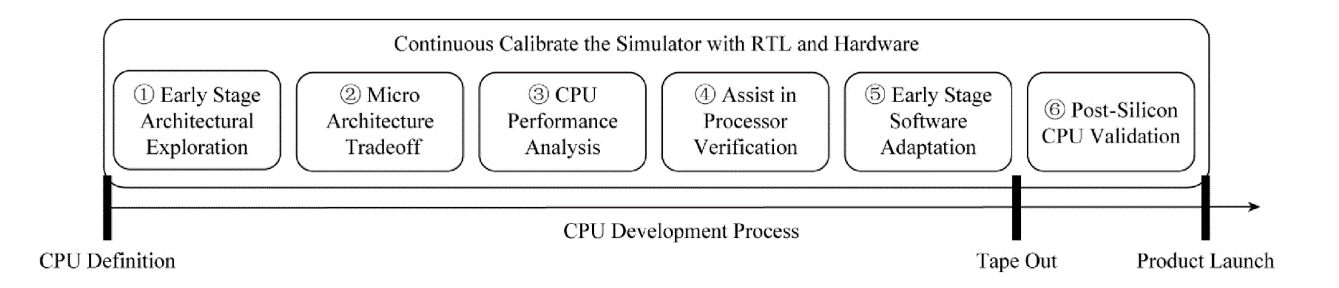
\includegraphics[width=1.0\textwidth]{simulator-func.png}
  \caption{体系结构模拟器在CPU开发流程中的作用}
  \label{fig:sim-func}
\end{figure}

\begin{figure}[h]
  \centering
  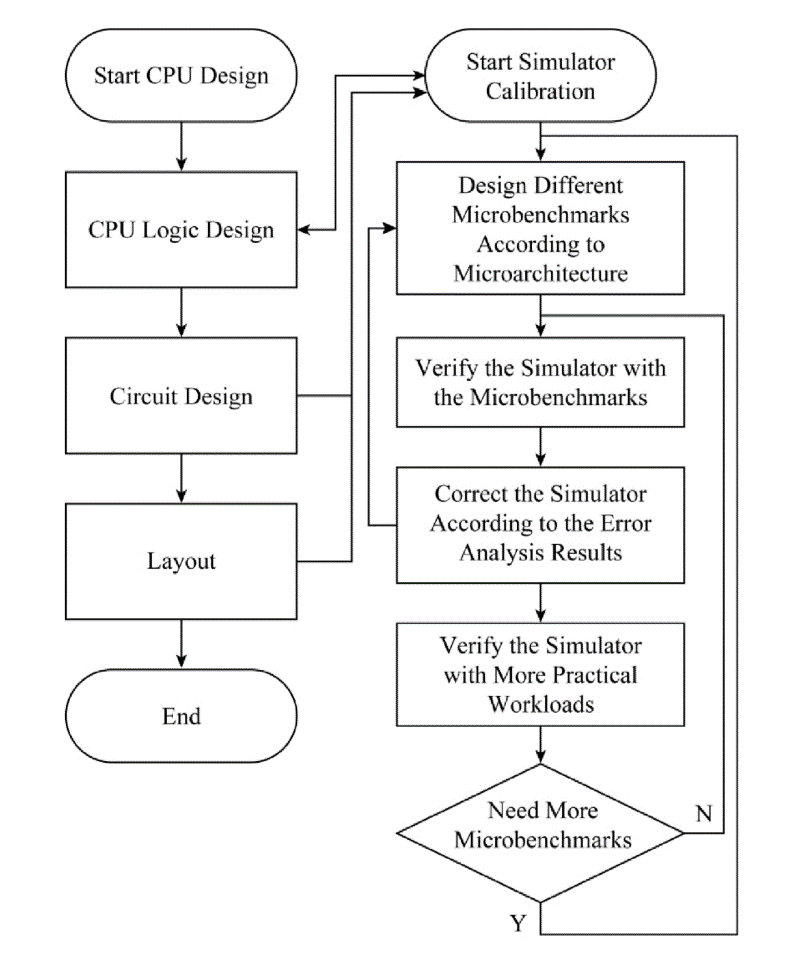
\includegraphics[width=0.6\textwidth]{simulator-develop-process.png}
  \caption{体系结构模拟器在CPU开发流程中的作用}
  \label{fig:sim-dev-process}
\end{figure}
模拟开发的基本流程如图~\ref{fig:sim-dev-process}所示

解释型指令集模拟器的工作流程很简单,通常是取指-译码-执行的循环,如图~\ref{fig:ISS-interprete}所示。
\begin{figure}[h]
  \centering
  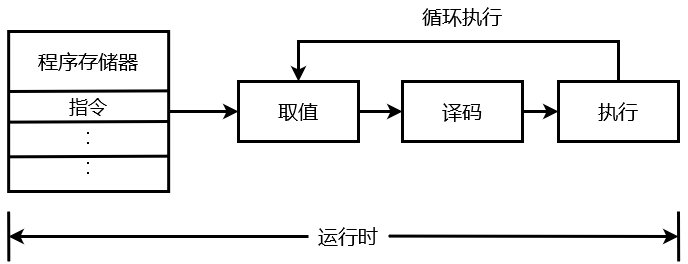
\includegraphics[width=0.9\textwidth]{ISS-interprete.png}
  \caption{体系结构模拟器在CPU开发流程中的作用}
  \label{fig:ISS-interprete}
\end{figure}

目标机二进制代码经编译器编译,之后由代码生成器优化生成宿主机的二进制代码,并最终运行于宿主机。
\begin{figure}[h]
  \centering
  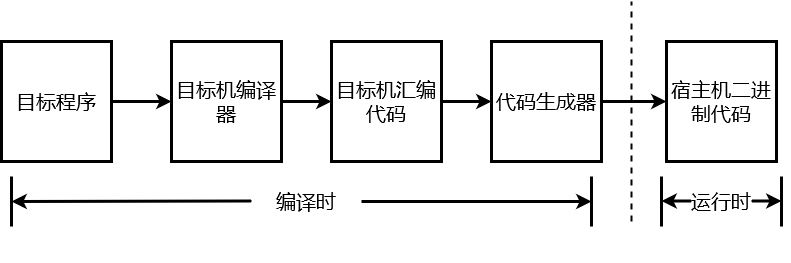
\includegraphics[width=0.9\textwidth]{static-ISS.png}
  \caption{体系结构模拟器在CPU开发流程中的作用}
  \label{fig:static-ISS}
\end{figure}


动态编译型指令集模拟器的典型代表为 Embra[33]及 Shade[34],其工作流程如图~\ref{fig:dynamic-ISS}所示:
\begin{figure}[h]
  \centering
  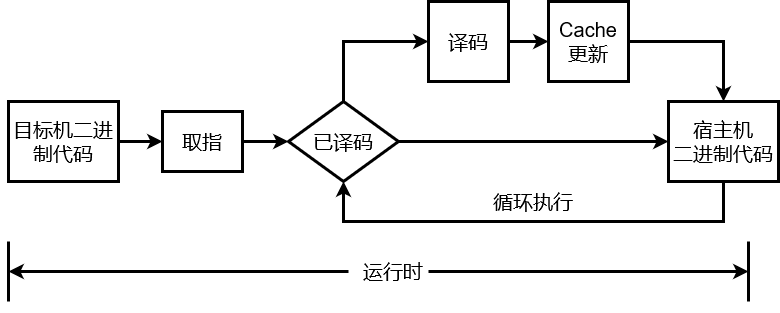
\includegraphics[width=0.9\textwidth]{dynamic-ISS.png}
  \caption{体系结构模拟器在CPU开发流程中的作用}
  \label{fig:dynamic-ISS}
\end{figure}


根据用例描述表可以得出系统软件开发/移植程序员的用例图如图~\ref{fig:badge}所示。
\begin{figure}[h]
  \centering
  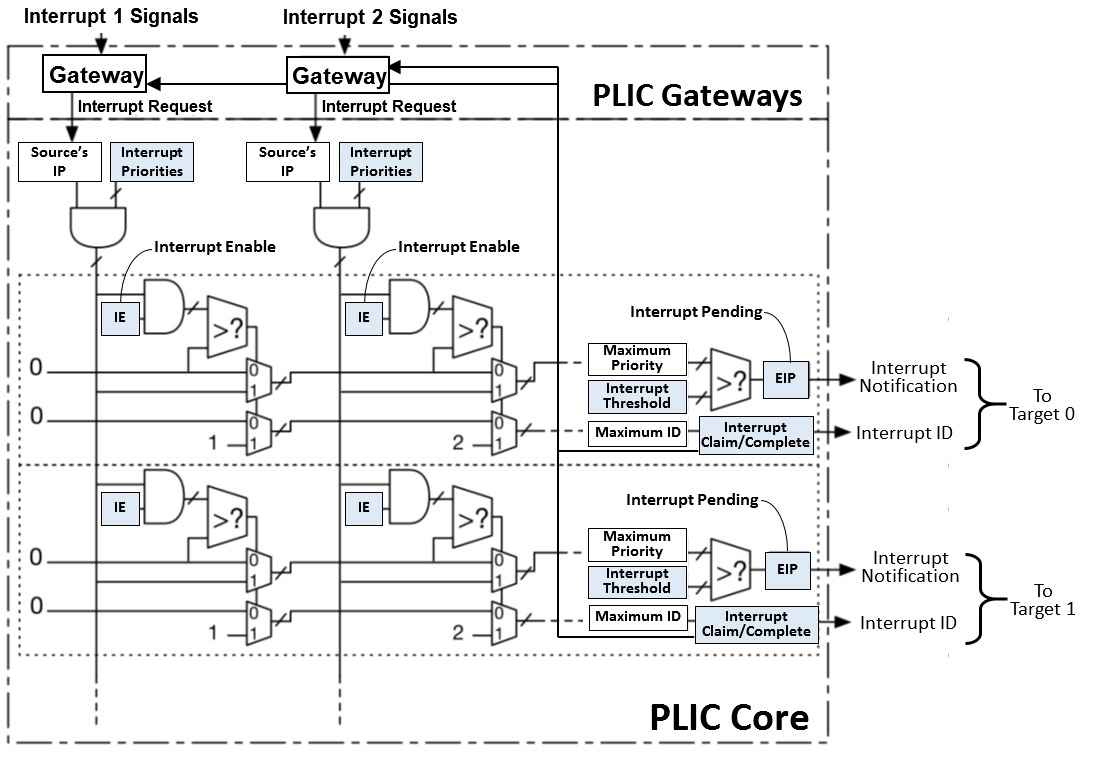
\includegraphics[width=0.7\textwidth]{PLICArch.jpg}
  \caption{图号、图题置于图的下方}
  \label{fig:badge}
\end{figure}

RISC-V指令集模拟器的整体功能模块如图\ref{fig:sim_general}所示
\begin{figure}[h]
  \centering
  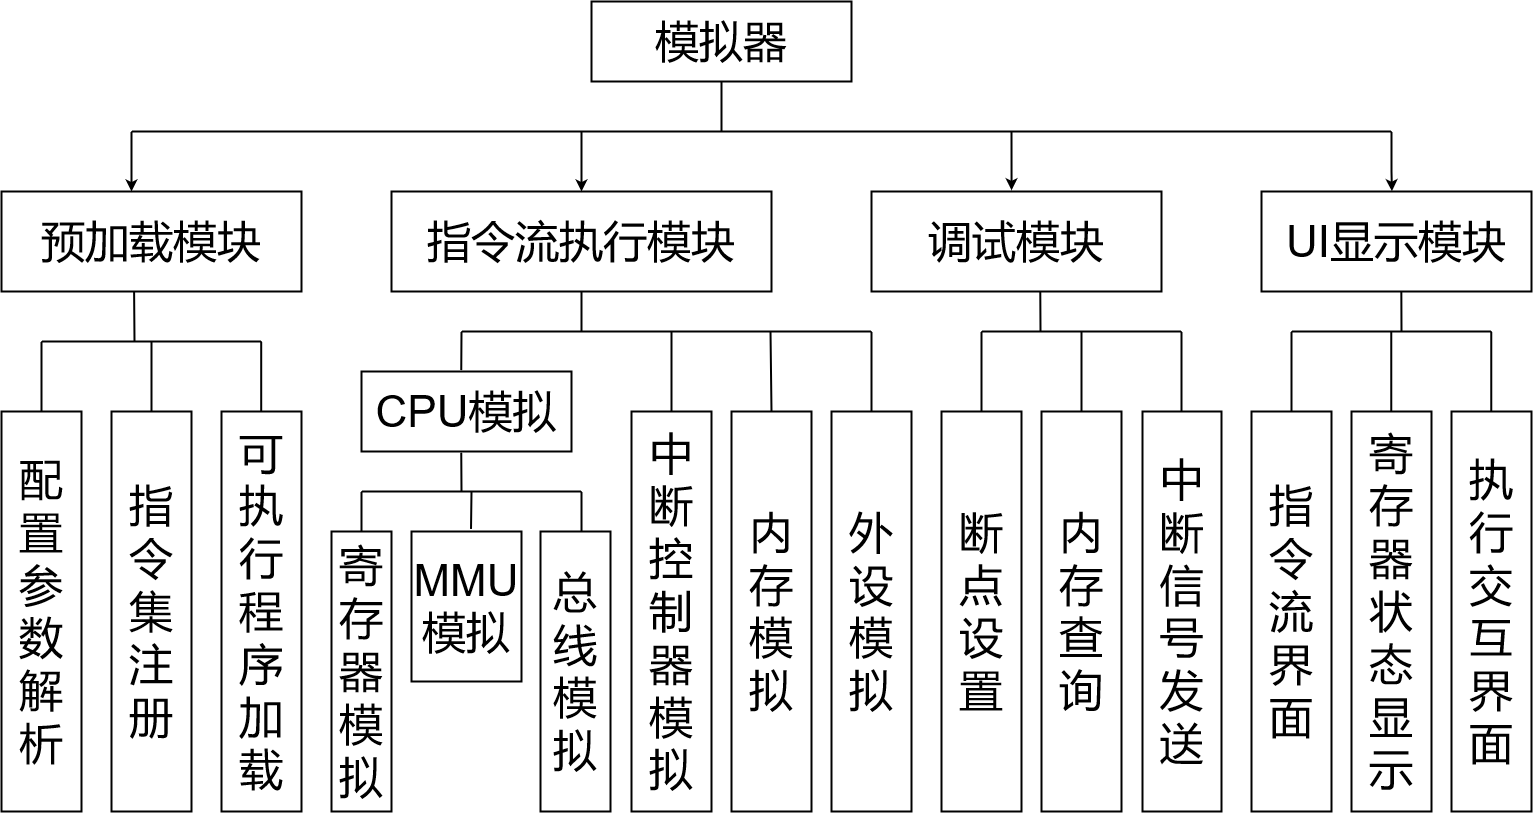
\includegraphics[width=1.0\textwidth]{sim-general.png}
  \caption{模拟器整体功能模块图}
  \label{fig:sim_general}
\end{figure}


\begin{figure}[h]
  \centering
  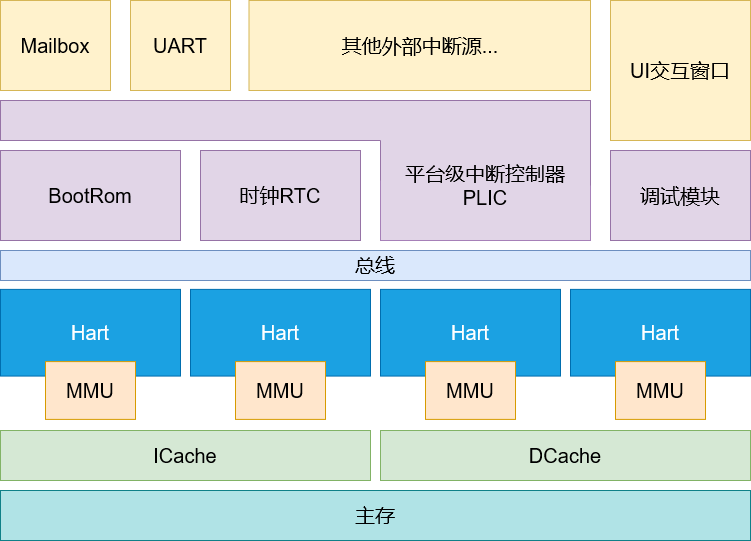
\includegraphics[width=0.8\textwidth]{cpu.png}
  \caption{处理器结构图}
  \label{fig:cpu}
\end{figure}
模拟出的RISC-V CPU整体架构如图\ref{fig:cpu}所示


\begin{figure}[h]
  \centering
  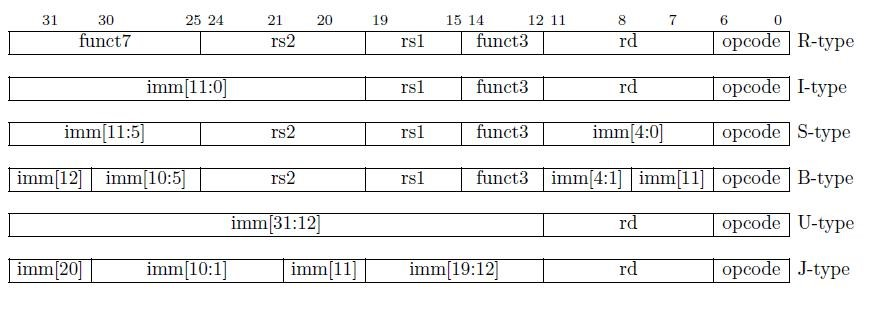
\includegraphics[width=1.0\textwidth]{insn-type.jpg}
  \caption{RISC-V32I 指令格式}
  \label{fig:insn-type}
\end{figure}
由前面的章节可以知道,RISC-V汇编指令的格式是非常明晰的,图~\ref{fig:insn-type}


\begin{figure}[h]
  \centering
  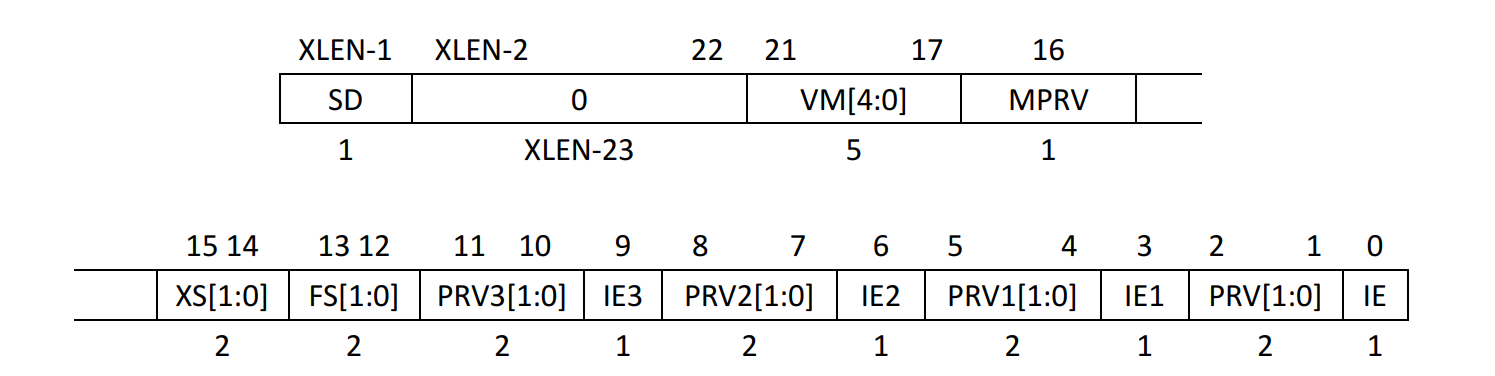
\includegraphics[width=0.8\textwidth]{mstatus.png}
  \caption{状态寄存器位域信息}
  \label{fig:mstatus}
\end{figure}
以状态寄存器CSR\_MSTATUS为例.如图~\ref{fig:mstatus}所示


图~\ref{fig:VM}给出了当前定义好的虚拟化方案。
\begin{figure}[h]
  \centering
  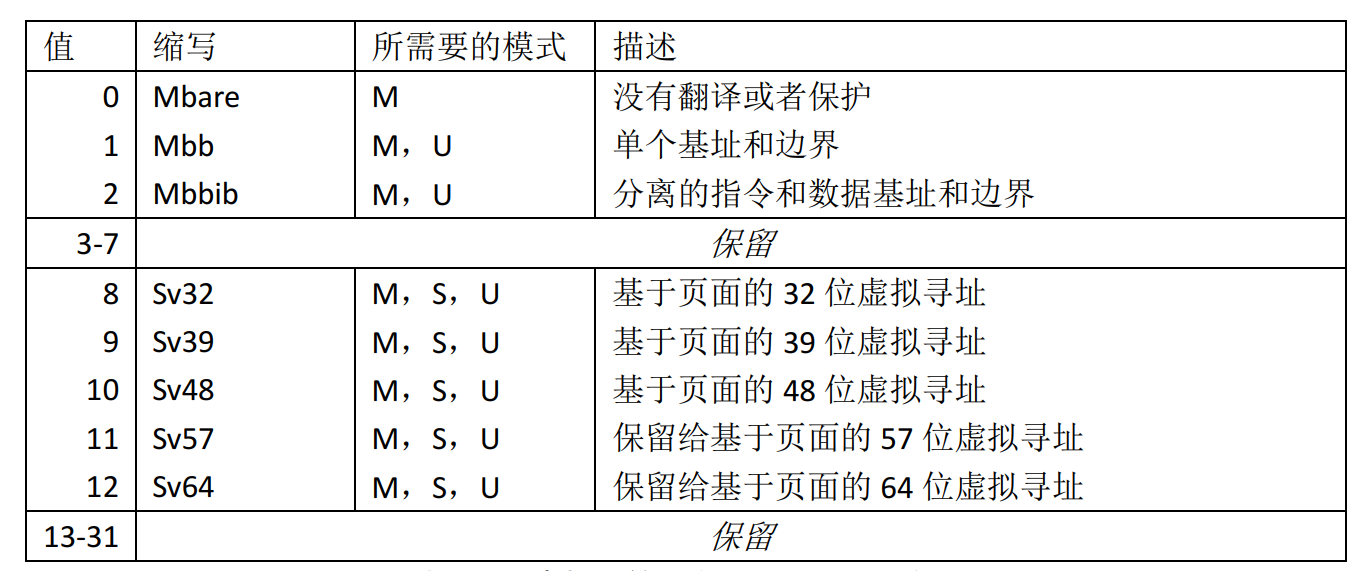
\includegraphics[width=0.8\textwidth]{VM.png}
  \caption{RISC-V虚拟化方案}
  \label{fig:VM}
\end{figure}

代码如下:
\begin{lstlisting}{}
  class trap_t
  {
  public:
      trap_t(){}
      trap_t(reg_t type):cause(type),addr_valid(false){}
      trap_t(reg_t type,quint64 addr):cause(type),addr_valid(true),addr(addr){}
      reg_t cause;
      bool addr_valid;
      quint64 addr;
      static QMap<reg_t,QString> names;
      static quint64 delegable_exceptions;
      QString &name(){return names[cause];}
  };        
\end{lstlisting}


测试用例设计如表~\ref{tab:demo}所示.
\begin{table}[h]
    \centering
    \caption{断点设置用例描述}
    \label{tab:demo}
    \begin{tabular}{clll}
      \toprule
      \multicolumn{1}{c}{序号} & \multicolumn{1}{c}{输入} & \multicolumn{1}{c}{预期输出} &\multicolumn{1}{c}{说明}\\
      \midrule
  1	& \multicolumn{1}{m{3.5cm}}{输入} & \multicolumn{1}{m{3.5cm}}{输入} & \multicolumn{1}{m{3.5cm}}{输入}\\
  \hline
  2	& \multicolumn{1}{m{3.5cm}}{输入} & \multicolumn{1}{m{3.5cm}}{输入} & \multicolumn{1}{m{3.5cm}}{输入}\\
  \hline
  3	& \multicolumn{1}{m{3.5cm}}{输入} & \multicolumn{1}{m{3.5cm}}{输入} & \multicolumn{1}{m{3.5cm}}{输入}\\
      \bottomrule
    \end{tabular}
\end{table}